
%%%%%%%%%%%%%%%%%%%%%%%%%%%%%%%%%%%%%%%%%%%%%%%%%%%%%%%%%%%
\section{Privacy Implications of Personal Data Processing} 
\label{sec:PrivacyImplicationsPersonalDataProcessing}
%%%%%%%%%%%%%%%%%%%%%%%%%%%%%%%%%%%%%%%%%%%%%%%%%%%%%%%%%%%


Data processing is the conversion of raw data to meaningful information through a process. Data is manipulated to produce results that lead to a resolution of a problem or improvement of an existing situation. 

Data Mining is the process of discovering interesting patterns and knowledge from large amounts of data \cite{han2011data}. We will describe the Data Mining process according to the widely used CRISP-DM model \cite{wirth2000crisp}, in which the process is separated into six major phases, as described next and in Figure \ref{fig:crisp-dm}.

\begin{itemize}
    \setlength\itemsep{1em}

    \item\textbf{Business Understanding:} In this initial phase, the project goals and requirements must be understood from a business perspective, and then converted into a Data Mining problem.

    \item\textbf{Data Understanding:} During this phase, an initial data collection is done, followed by a number of activities in order to get familiar with the data, to understand how the data is organized, to identify if the data has quality problems, or even to detect interesting subsets in the data collected.

    \item\textbf{Data Preparation:} This phase covers all the data preparation tasks to construct the final dataset from the initial raw data collected. These tasks include attribute selection, data cleaning, and transformation of data to fit the modeling tools.

    \item\textbf{Modeling:} In this phase, various modeling techniques are selected and applied, and the underlying parameters are calibrated to optimal values. Usually, there are several techniques for the same Data Mining problem type, and some of these techniques require specific data formats.

    \item\textbf{Evaluation:} At this point in the Data Mining process, one or more models have been developed that appear to have high quality, from a data analysis perspective. These models must be evaluated thoroughly so that we can be certain that they properly achieve the business goals.

    \item\textbf{Deployment:} In this last phase, the knowledge gained by the Data Mining process will need to be organized and presented in a way that the customer can use it. This, of course, depends on the requirements presented at the beginning of the process. An example of a common deployment that results from Data Mining is a simple report on the knowledge obtained. 

\end{itemize}

\begin{figure}[!ht]
  \centering
  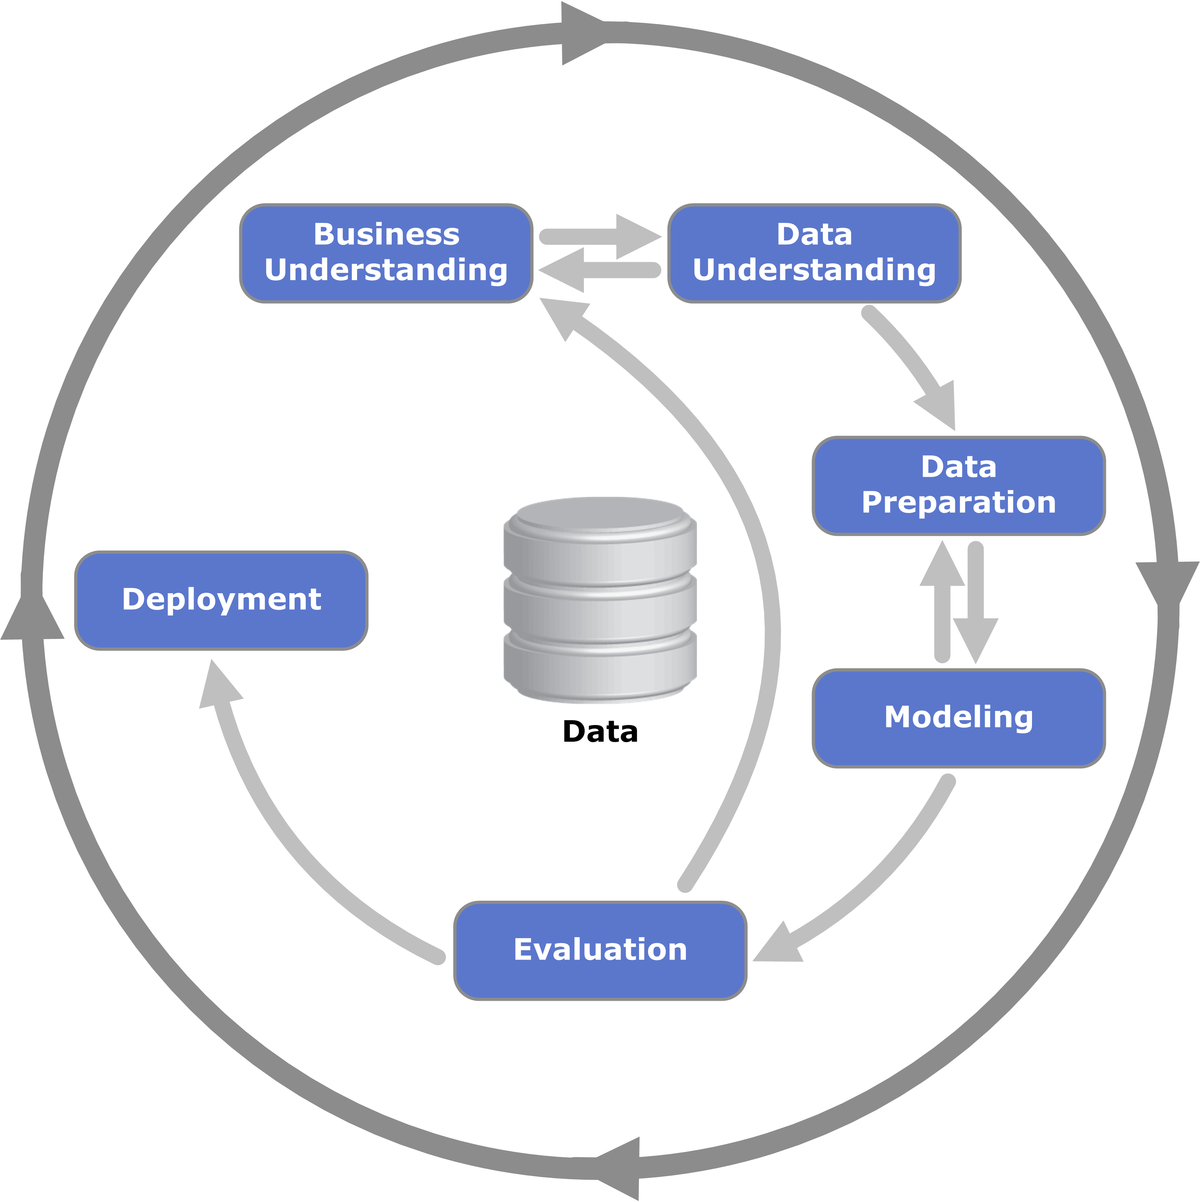
\includegraphics[width=0.60\textwidth]{images/CRISP-DM_Process_Diagram.png}
  \caption{Process diagram showing the relationship between the different phases of CRISP-DM \cite{wirth2000crisp}.}
  \label{fig:crisp-dm}
\end{figure}



In the Data Mining process, we must be aware that, sometimes, private information about individuals can be used and it may lead to breaches of privacy. We define this private information as \ac{pii} or \ac{spi} \cite{schwartz2011pii}. This concept can be defined as information that can be used alone or in conjunction with other information to identify, contact, or locate a single person, or to identify an individual in a context.



%%%%%%%%%%%%%%%%%%%%%%%%%%%%%%%%%%%%%%%%%%%%%%
\subsection{Attack Models}
\label{ssec:AttackModels}
%%%%%%%%%%%%%%%%%%%%%%%%%%%%%%%%%%%%%%%%%%%%%%

When considering the security of a system, one must have into account the concepts of threat model, attack model, and the two types of adversaries, \textit{honest-but-curious} and \textit{malicious}, to understand how to better implement an efficient and trustworthy security layer.

A threat model specifies the potential threats that can be used against a system, by identifying, enumerating and prioritizing them. A well known and defined threat assessment model is the STRIDE model developed by Microsoft \cite{hafiz2007organizing}.

Cryptographic attacks are used whenever the target system relies on cryptography for protection. An attack model is, in terms of cryptanalysis, a classification of cryptographic attacks specifying the type of access the attacker has to a system when attempting to break an encrypted message. We can summarize the cryptographic attack in the following four categories:

 \begin{itemize}
    \setlength\itemsep{1em}

    \item \textbf{Ciphertext-only attack:} In this type of attack, the cryptanalyst has access only to the ciphertext and has no access to the plaintext. This is the most common type of attack, and it is a requirement for modern ciphers to be resistant to it. An example of a ciphertext-only attack is the brute force attack, where the attacker makes a trial-and-error approach to decrypt the ciphertext.

    \item \textbf{Known-plaintext attack:} In this type of attack, the cryptanalyst has access to a number of pairs of plaintext and the corresponding ciphertext.

    \item \textbf{Chosen-plaintext attack:} In this type of attack, the cryptanalyst is able to encrypt arbitrary plaintext and have access to the resulting ciphertext, allowing him to make a statistical analysis on the plaintext state space.

    \item \textbf{Chosen-ciphertext attack:} In this type of attack, the cryptanalyst is able to choose arbitrary ciphertext and obtain the corresponding plaintext.
\end{itemize}


We can also classify the types of adversaries according to their strategies in two major groups: \textit{honest-but-curious} and \textit{malicious} adversaries.
The honest-but-curious adversary follows the protocol in plan, but he will try to extract information from his viewpoint of the protocol to gain some form of advantage or gain access to confidential information.
The malicious adversary is one that can deviate from the protocol specification as he desires, and will try to disrupt and/or collect as many information as he can.

%
%Two different trust models can be considered when developing a system: \textit{semi-honest(honest-but-curious) security}, where we assume corrupted parties just gather information they can reach, they do not deviate from the protocol; and \textit{malicious security}, in which we assume corrupted parties can disrupt the protocol execution.

